%- block legend

% o jugisto nao aceita wrap AAAAAAA
% e nem parbox kkkkrying

\begin{center}
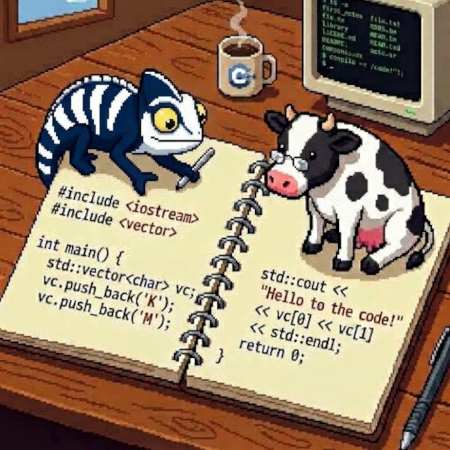
\includegraphics[width=0.2\linewidth]{maratona.png}
\end{center}

Pensando em estar sempre preparada para as Maratonas de Programação que
ocorrem durante o ano, sua equipe está montando seu material
de consulta. O material contém a implementação pronta de $N$ algoritmos
diferentes, que sua equipe sempre leva impressa para as provas para consultar.

O material tem $N$ páginas. Tanto os algoritmos quanto as páginas são numerados
de $1$ a $N$.
Inicialmente, o algoritmo $i$ estava na página $i$ ($1 \leq i \leq N$).

Entretanto, sua equipe decidiu fazer $M$ operações no material.
Em cada operação, a equipe inverteu a ordem dos
algoritmos entre as páginas $L_i$ e $R_i$, inclusive.
Sua equipe acredita que, fazendo isso, o material fica mais organizado.

Temos outra Maratona amanhã, na
LATINOWARE em Foz do Iguaçu, e sua equipe precisa do material de consulta
atualizado para levar para a competição.
Por isso, determine a ordem na qual os algoritmos ficaram no material, após
todas as operações feitas pela equipe, ainda hoje!

%- endblock

%- block input
A primeira linha contém dois inteiros $N$ e $M$
($\VAR{N.min} \leq N \leq \VAR{N.max | sci}$,
$\VAR{M.min} \leq M \leq \VAR{M.max | sci}$),
o número de algoritmos e páginas, e o número de operações feitas.
As próximas $M$ linhas descrevem uma operação cada, na ordem em que foram
feitas. Cada linha contém dois inteiros $L_i$ e $R_i$
($1 \leq L_i \leq R_i \leq N$).
%- endblock

%- block output
Imprima uma linha com $N$ inteiros, indicando a ordem final dos algoritmos no
material de consulta.
%- endblock

%- block explanation_0
No exemplo de entrada, as seguintes operações serão feitas:
\begin{itemize}
    \item $[1,\underline{2,3},4,5,6]$ $\rightarrow$ $[1,3,2,4,5,6]$
    \item $[1,3,\underline{2,4,5,6}]$ $\rightarrow$ $[1,3,6,5,4,2]$
    \item $[1,\underline{3,6,5},4,2]$ $\rightarrow$ $[1,5,6,3,4,2]$
\end{itemize}
%- endblock

%- block editorial
O problema pode ser resolvido com uma \textit{árvore cartesiana}, também chamada
de \textit{treap}. A \textit{treap} é uma árvore binária em que cada nó contém, além de sua
chave em si, uma coordenada $(x,y)$. Em relação aos valores $x$, a árvore se comporta como uma
árvore binária de busca (BST). Em relação aos valores $y$, a árvore se comporta como
uma \textit{heap}.

Neste problema, o valor de $x$ será o índice de uma página,
enquanto a chave em si é o algoritmo atualmente nesta
página. Neste caso, o valor de $x$ não é armazenado no nó, mas sim calculado
implicitamente durante as operações na estrutura. Além disso, o valor de
$y$ pode ser um inteiro \textit{gerado aleatória e uniformemente}, o que
garante, na prática, a altura logarítmica da árvore
(pois a probabilidade de $h \neq O(\lg N)$, para valores grandes e relevantes
de $N$, é virtualmente nula).

Você pode ler mais sobre a \textit{treap} em \url{https://cp-algorithms.com/data\_structures/treap.html}.

Para cada operação $(L_i, R_i)$, realize um \textit{split} para $x < L_i$ e outro para $x
\leq R_i$. Isto gera três árvores $A$, $B$ e $C$, de forma que ``isolamos'', na
árvore $B$, os nós cujas posições $x$ estão entre $L_i$ e $R_i$.
A figura abaixo mostra uma \textit{treap}, os \textit{splits} feitos para
$L_i=2$ e $R_i=3$ e as três árvores resultantes.

\begin{center}
    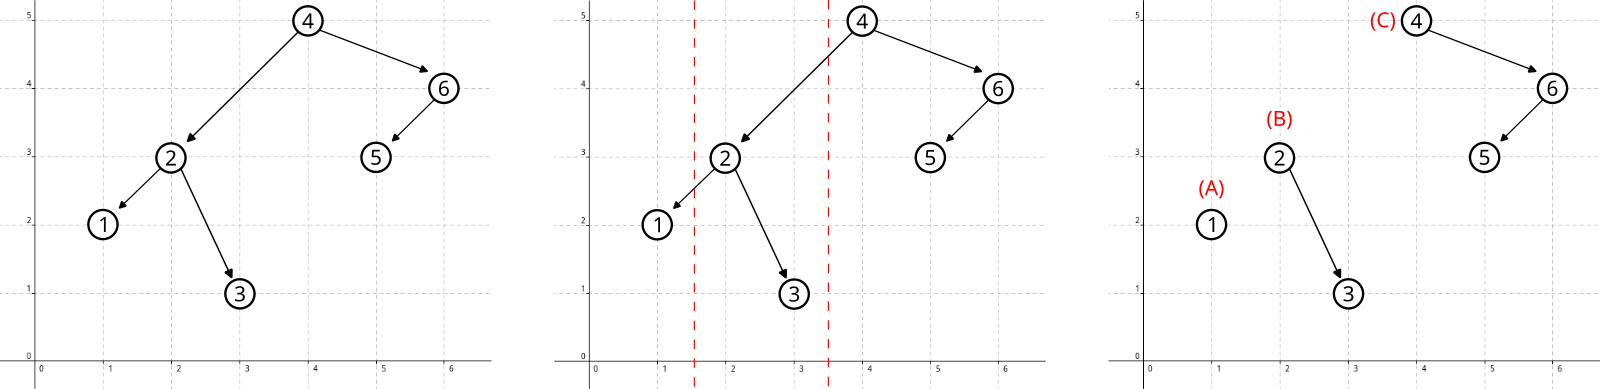
\includegraphics[scale=0.3]{editorial.png}
\end{center}

Agora, precisamos inverter a ordem das chaves em toda a subárvore $B$, e fazer duas operações
\textit{merge} para reconstruir toda a árvore.

\begin{center}
    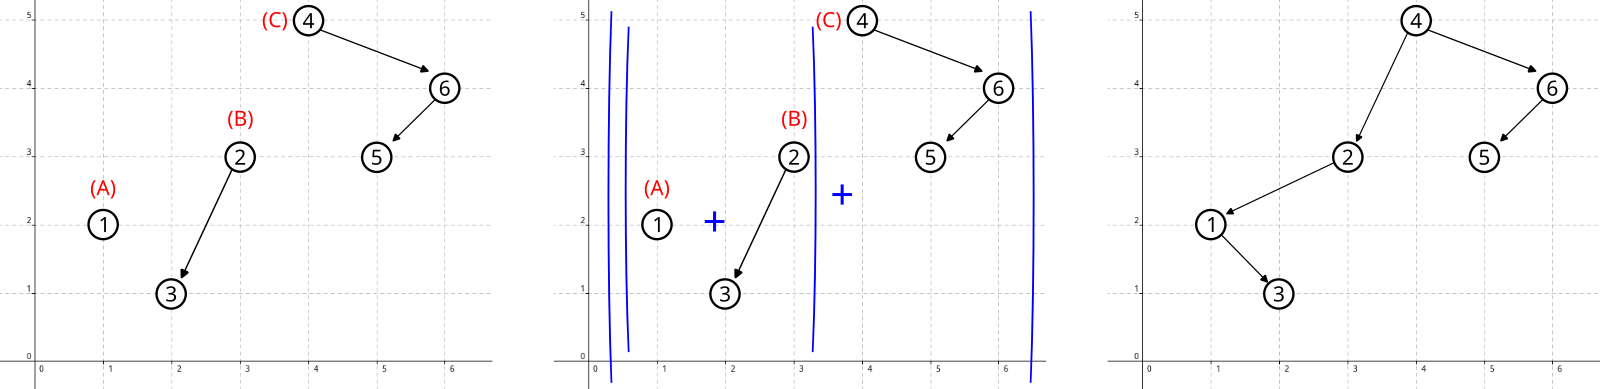
\includegraphics[scale=0.3]{editorial2.png}
\end{center}

Para inverter a árvore $B$ eficientemente, utilize a técnica de \textit{lazy propagation}:
mantenha em cada nó uma \textit{flag}
indicando se a subárvore enraizada nele deve ser invertida. Coloque a
\textit{flag} na raíz da árvore $B$. Então, sempre que um nó for visitado
durante qualquer operação, verifique sua \textit{flag} e, se
necessário, troque os ponteiros para seus filhos e ``empurre'' a
\textit{flag} para ambos.

Por fim, faça um percurso \textit{in-order} na árvore final para imprimir a
resposta.

Complexidade total: $O((N+Q)\lg N)$ (com probabilidade virtualmente garantida).

%- endblock
